\chapter{Sorting}

\index{sorting}

\key{Sorting}
is a fundamental algorithm design problem.
Many efficient algorithms
use sorting as a subroutine,
because it is often easier to process
data if the elements are in a sorted order.

For example, the problem ''does an array contain
two equal elements?'' is easy to solve using sorting.
If the array contains two equal elements,
they will be next to each other after sorting,
so it is easy to find them.
Also, the problem ''what is the most frequent element
in an array?'' can be solved similarly.

There are many algorithms for sorting, and they are
also good examples of how to apply
different algorithm design techniques.
The efficient general sorting algorithms
work in $O(n \log n)$ time,
and many algorithms that use sorting
as a subroutine also
have this time complexity.

\section{Sorting theory}

The basic problem in sorting is as follows:
\begin{framed}
\noindent
Given an array that contains $n$ elements,
your task is to sort the elements
in increasing order.
\end{framed}
\noindent
For example, the array
\begin{center}
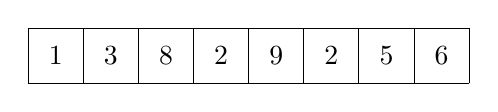
\begin{tikzpicture}[scale=0.7]
\draw (0,0) grid (8,1);
\node at (0.5,0.5) {$1$};
\node at (1.5,0.5) {$3$};
\node at (2.5,0.5) {$8$};
\node at (3.5,0.5) {$2$};
\node at (4.5,0.5) {$9$};
\node at (5.5,0.5) {$2$};
\node at (6.5,0.5) {$5$};
\node at (7.5,0.5) {$6$};
\end{tikzpicture}
\end{center}
will be as follows after sorting:
\begin{center}
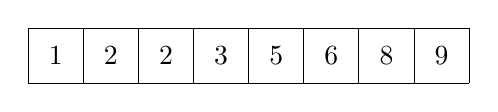
\begin{tikzpicture}[scale=0.7]
\draw (0,0) grid (8,1);
\node at (0.5,0.5) {$1$};
\node at (1.5,0.5) {$2$};
\node at (2.5,0.5) {$2$};
\node at (3.5,0.5) {$3$};
\node at (4.5,0.5) {$5$};
\node at (5.5,0.5) {$6$};
\node at (6.5,0.5) {$8$};
\node at (7.5,0.5) {$9$};
\end{tikzpicture}
\end{center}

\subsubsection{$O(n^2)$ algorithms}

\index{bubble sort}

Simple algorithms for sorting an array
work in $O(n^2)$ time.
Such algorithms are short and usually
consist of two nested loops.
A famous $O(n^2)$ time sorting algorithm
is \key{bubble sort} where the elements
''bubble'' in the array according to their values.

Bubble sort consists of $n$ rounds.
On each round, the algorithm iterates through
the elements of the array.
Whenever two consecutive elements are found
that are not in correct order,
the algorithm swaps them.
The algorithm can be implemented as follows:
\begin{lstlisting}
for i in 0..n {
    for j in 0..n-1 {
        if array[j] > array[j+1] {
            array.swap(j, j+1);
        }
    }
}
\end{lstlisting}

After the first round of the algorithm,
the largest element will be in the correct position,
and in general, after $k$ rounds, the $k$ largest
elements will be in the correct positions.
Thus, after $n$ rounds, the whole array
will be sorted.

For example, in the array

\begin{center}
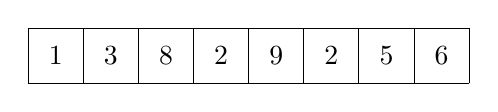
\begin{tikzpicture}[scale=0.7]
\draw (0,0) grid (8,1);

\node at (0.5,0.5) {$1$};
\node at (1.5,0.5) {$3$};
\node at (2.5,0.5) {$8$};
\node at (3.5,0.5) {$2$};
\node at (4.5,0.5) {$9$};
\node at (5.5,0.5) {$2$};
\node at (6.5,0.5) {$5$};
\node at (7.5,0.5) {$6$};
\end{tikzpicture}
\end{center}

\noindent
the first round of bubble sort swaps elements
as follows:

\begin{center}
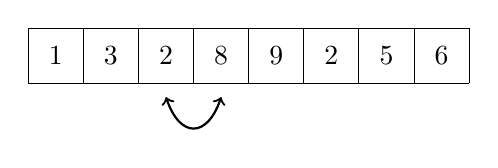
\begin{tikzpicture}[scale=0.7]
\draw (0,0) grid (8,1);
\node at (0.5,0.5) {$1$};
\node at (1.5,0.5) {$3$};
\node at (2.5,0.5) {$2$};
\node at (3.5,0.5) {$8$};
\node at (4.5,0.5) {$9$};
\node at (5.5,0.5) {$2$};
\node at (6.5,0.5) {$5$};
\node at (7.5,0.5) {$6$};

\draw[thick,<->] (3.5,-0.25) .. controls (3.25,-1.00) and (2.75,-1.00) .. (2.5,-0.25);
\end{tikzpicture}
\end{center}

\begin{center}
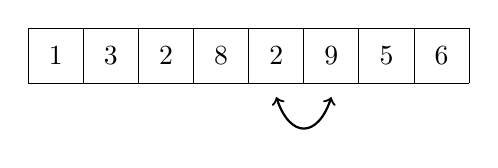
\begin{tikzpicture}[scale=0.7]
\draw (0,0) grid (8,1);
\node at (0.5,0.5) {$1$};
\node at (1.5,0.5) {$3$};
\node at (2.5,0.5) {$2$};
\node at (3.5,0.5) {$8$};
\node at (4.5,0.5) {$2$};
\node at (5.5,0.5) {$9$};
\node at (6.5,0.5) {$5$};
\node at (7.5,0.5) {$6$};

\draw[thick,<->] (5.5,-0.25) .. controls (5.25,-1.00) and (4.75,-1.00) .. (4.5,-0.25);
\end{tikzpicture}
\end{center}

\begin{center}
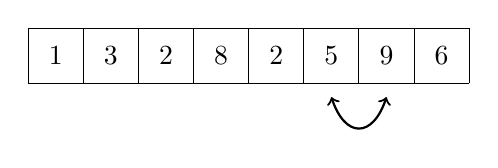
\begin{tikzpicture}[scale=0.7]
\draw (0,0) grid (8,1);
\node at (0.5,0.5) {$1$};
\node at (1.5,0.5) {$3$};
\node at (2.5,0.5) {$2$};
\node at (3.5,0.5) {$8$};
\node at (4.5,0.5) {$2$};
\node at (5.5,0.5) {$5$};
\node at (6.5,0.5) {$9$};
\node at (7.5,0.5) {$6$};

\draw[thick,<->] (6.5,-0.25) .. controls (6.25,-1.00) and (5.75,-1.00) .. (5.5,-0.25);
\end{tikzpicture}
\end{center}

\begin{center}
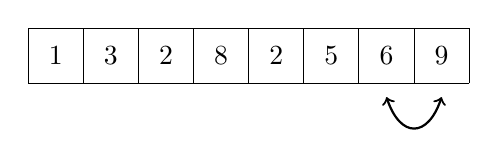
\begin{tikzpicture}[scale=0.7]
\draw (0,0) grid (8,1);
\node at (0.5,0.5) {$1$};
\node at (1.5,0.5) {$3$};
\node at (2.5,0.5) {$2$};
\node at (3.5,0.5) {$8$};
\node at (4.5,0.5) {$2$};
\node at (5.5,0.5) {$5$};
\node at (6.5,0.5) {$6$};
\node at (7.5,0.5) {$9$};

\draw[thick,<->] (7.5,-0.25) .. controls (7.25,-1.00) and (6.75,-1.00) .. (6.5,-0.25);
\end{tikzpicture}
\end{center}

\subsubsection{Inversions}

\index{inversion}

Bubble sort is an example of a sorting
algorithm that always swaps \emph{consecutive}
elements in the array.
It turns out that the time complexity
of such an algorithm is \emph{always}
at least $O(n^2)$, because in the worst case,
$O(n^2)$ swaps are required for sorting the array.

A useful concept when analyzing sorting
algorithms is an \key{inversion}:
a pair of array elements
$(\texttt{array}[a],\texttt{array}[b])$ such that
$a<b$ and $\texttt{array}[a]>\texttt{array}[b]$,
i.e., the elements are in the wrong order.
For example, the array
\begin{center}
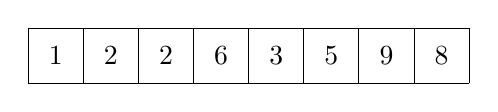
\begin{tikzpicture}[scale=0.7]
\draw (0,0) grid (8,1);
\node at (0.5,0.5) {$1$};
\node at (1.5,0.5) {$2$};
\node at (2.5,0.5) {$2$};
\node at (3.5,0.5) {$6$};
\node at (4.5,0.5) {$3$};
\node at (5.5,0.5) {$5$};
\node at (6.5,0.5) {$9$};
\node at (7.5,0.5) {$8$};
\end{tikzpicture}
\end{center}
has three inversions: $(6,3)$, $(6,5)$ and $(9,8)$.
The number of inversions indicates
how much work is needed to sort the array.
An array is completely sorted when
there are no inversions.
On the other hand, if the array elements
are in the reverse order,
the number of inversions is the largest possible:
\[1+2+\cdots+(n-1)=\frac{n(n-1)}{2} = O(n^2)\]

Swapping a pair of consecutive elements that are
in the wrong order removes exactly one inversion
from the array.
Hence, if a sorting algorithm can only
swap consecutive elements, each swap removes
at most one inversion, and the time complexity
of the algorithm is at least $O(n^2)$.

\subsubsection{$O(n \log n)$ algorithms}

\index{merge sort}

It is possible to sort an array efficiently
in $O(n \log n)$ time using algorithms
that are not limited to swapping consecutive elements.
One such algorithm is \key{merge sort}\footnote{According to \cite{knu983},
merge sort was invented by J. von Neumann in 1945.},
which is based on recursion.

Merge sort sorts a subarray \texttt{array}$[a \ldots b]$ as follows:

\begin{enumerate}
\item If $a=b$, do not do anything, because the subarray is already sorted.
\item Calculate the position of the middle element: $k=\lfloor (a+b)/2 \rfloor$.
\item Recursively sort the subarray \texttt{array}$[a \ldots k]$.
\item Recursively sort the subarray \texttt{array}$[k+1 \ldots b]$.
\item \emph{Merge} the sorted subarrays \texttt{array}$[a \ldots k]$ and
\texttt{array}$[k+1 \ldots b]$
into a sorted subarray \texttt{array}$[a \ldots b]$.
\end{enumerate}

Merge sort is an efficient algorithm, because it
halves the size of the subarray at each step.
The recursion consists of $O(\log n)$ levels,
and processing each level takes $O(n)$ time.
Merging the subarrays \texttt{array}$[a \ldots k]$ and \texttt{array}$[k+1 \ldots b]$
is possible in linear time, because they are already sorted.

For example, consider sorting the following array:
\begin{center}
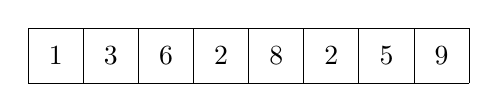
\begin{tikzpicture}[scale=0.7]
\draw (0,0) grid (8,1);
\node at (0.5,0.5) {$1$};
\node at (1.5,0.5) {$3$};
\node at (2.5,0.5) {$6$};
\node at (3.5,0.5) {$2$};
\node at (4.5,0.5) {$8$};
\node at (5.5,0.5) {$2$};
\node at (6.5,0.5) {$5$};
\node at (7.5,0.5) {$9$};
\end{tikzpicture}
\end{center}

The array will be divided into two subarrays
as follows:
\begin{center}
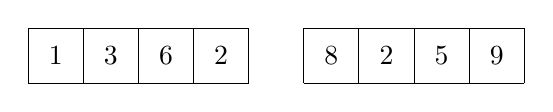
\begin{tikzpicture}[scale=0.7]
\draw (0,0) grid (4,1);
\draw (5,0) grid (9,1);

\node at (0.5,0.5) {$1$};
\node at (1.5,0.5) {$3$};
\node at (2.5,0.5) {$6$};
\node at (3.5,0.5) {$2$};

\node at (5.5,0.5) {$8$};
\node at (6.5,0.5) {$2$};
\node at (7.5,0.5) {$5$};
\node at (8.5,0.5) {$9$};
\end{tikzpicture}
\end{center}

Then, the subarrays will be sorted recursively
as follows:
\begin{center}
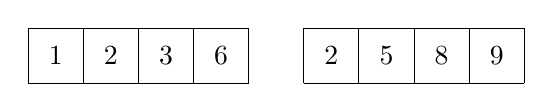
\begin{tikzpicture}[scale=0.7]
\draw (0,0) grid (4,1);
\draw (5,0) grid (9,1);

\node at (0.5,0.5) {$1$};
\node at (1.5,0.5) {$2$};
\node at (2.5,0.5) {$3$};
\node at (3.5,0.5) {$6$};

\node at (5.5,0.5) {$2$};
\node at (6.5,0.5) {$5$};
\node at (7.5,0.5) {$8$};
\node at (8.5,0.5) {$9$};
\end{tikzpicture}
\end{center}

Finally, the algorithm merges the sorted
subarrays and creates the final sorted array:
\begin{center}
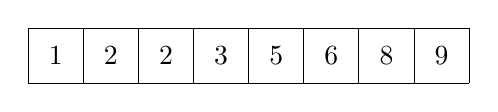
\begin{tikzpicture}[scale=0.7]
\draw (0,0) grid (8,1);
\node at (0.5,0.5) {$1$};
\node at (1.5,0.5) {$2$};
\node at (2.5,0.5) {$2$};
\node at (3.5,0.5) {$3$};
\node at (4.5,0.5) {$5$};
\node at (5.5,0.5) {$6$};
\node at (6.5,0.5) {$8$};
\node at (7.5,0.5) {$9$};
\end{tikzpicture}
\end{center}

\subsubsection{Sorting lower bound}

Is it possible to sort an array faster
than in $O(n \log n)$ time?
It turns out that this is \emph{not} possible
when we restrict ourselves to sorting algorithms
that are based on comparing array elements.

The lower bound for the time complexity
can be proved by considering sorting
as a process where each comparison of two elements
gives more information about the contents of the array.
The process creates the following tree:

\begin{center}
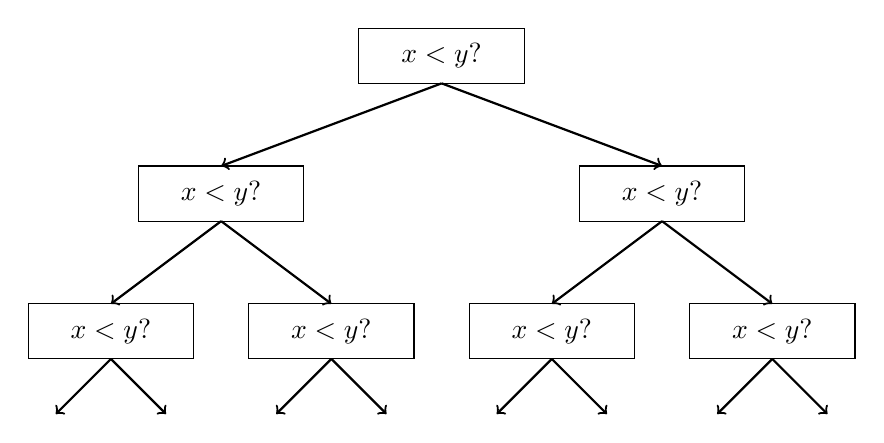
\begin{tikzpicture}[scale=0.7]
\draw (0,0) rectangle (3,1);
\node at (1.5,0.5) {$x < y?$};

\draw[thick,->] (1.5,0) -- (-2.5,-1.5);
\draw[thick,->] (1.5,0) -- (5.5,-1.5);

\draw (-4,-2.5) rectangle (-1,-1.5);
\draw (4,-2.5) rectangle (7,-1.5);
\node at (-2.5,-2) {$x < y?$};
\node at (5.5,-2) {$x < y?$};

\draw[thick,->] (-2.5,-2.5) -- (-4.5,-4);
\draw[thick,->] (-2.5,-2.5) -- (-0.5,-4);
\draw[thick,->] (5.5,-2.5) -- (3.5,-4);
\draw[thick,->] (5.5,-2.5) -- (7.5,-4);

\draw (-6,-5) rectangle (-3,-4);
\draw (-2,-5) rectangle (1,-4);
\draw (2,-5) rectangle (5,-4);
\draw (6,-5) rectangle (9,-4);
\node at (-4.5,-4.5) {$x < y?$};
\node at (-0.5,-4.5) {$x < y?$};
\node at (3.5,-4.5) {$x < y?$};
\node at (7.5,-4.5) {$x < y?$};

\draw[thick,->] (-4.5,-5) -- (-5.5,-6);
\draw[thick,->] (-4.5,-5) -- (-3.5,-6);
\draw[thick,->] (-0.5,-5) -- (0.5,-6);
\draw[thick,->] (-0.5,-5) -- (-1.5,-6);
\draw[thick,->] (3.5,-5) -- (2.5,-6);
\draw[thick,->] (3.5,-5) -- (4.5,-6);
\draw[thick,->] (7.5,-5) -- (6.5,-6);
\draw[thick,->] (7.5,-5) -- (8.5,-6);
\end{tikzpicture}
\end{center}

Here ''$x<y?$'' means that some elements
$x$ and $y$ are compared.
If $x<y$, the process continues to the left,
and otherwise to the right.
The results of the process are the possible
ways to sort the array, a total of $n!$ ways.
For this reason, the height of the tree
must be at least
\[ \log_2(n!) = \log_2(1)+\log_2(2)+\cdots+\log_2(n).\]
We get a lower bound for this sum
by choosing the last $n/2$ elements and
changing the value of each element to $\log_2(n/2)$.
This yields an estimate
\[ \log_2(n!) \ge (n/2) \cdot \log_2(n/2),\]
so the height of the tree and the minimum
possible number of steps in a sorting
algorithm in the worst case
is at least $n \log n$.

\subsubsection{Counting sort}

\index{counting sort}

The lower bound $n \log n$ does not apply to
algorithms that do not compare array elements
but use some other information.
An example of such an algorithm is
\key{counting sort} that sorts an array in
$O(n)$ time assuming that every element in the array
is an integer between $0 \ldots c$ and $c=O(n)$.

The algorithm creates a \emph{bookkeeping} array,
whose indices are elements of the original array.
The algorithm iterates through the original array
and calculates how many times each element
appears in the array.
\newpage

For example, the array
\begin{center}
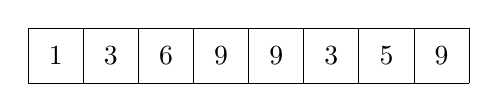
\begin{tikzpicture}[scale=0.7]
\draw (0,0) grid (8,1);
\node at (0.5,0.5) {$1$};
\node at (1.5,0.5) {$3$};
\node at (2.5,0.5) {$6$};
\node at (3.5,0.5) {$9$};
\node at (4.5,0.5) {$9$};
\node at (5.5,0.5) {$3$};
\node at (6.5,0.5) {$5$};
\node at (7.5,0.5) {$9$};
\end{tikzpicture}
\end{center}
corresponds to the following bookkeeping array:
\begin{center}
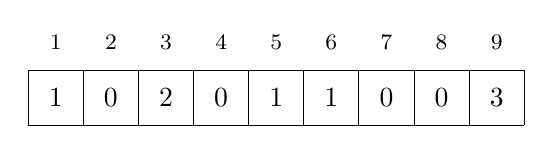
\begin{tikzpicture}[scale=0.7]
\draw (0,0) grid (9,1);
\node at (0.5,0.5) {$1$};
\node at (1.5,0.5) {$0$};
\node at (2.5,0.5) {$2$};
\node at (3.5,0.5) {$0$};
\node at (4.5,0.5) {$1$};
\node at (5.5,0.5) {$1$};
\node at (6.5,0.5) {$0$};
\node at (7.5,0.5) {$0$};
\node at (8.5,0.5) {$3$};

\footnotesize

\node at (0.5,1.5) {$1$};
\node at (1.5,1.5) {$2$};
\node at (2.5,1.5) {$3$};
\node at (3.5,1.5) {$4$};
\node at (4.5,1.5) {$5$};
\node at (5.5,1.5) {$6$};
\node at (6.5,1.5) {$7$};
\node at (7.5,1.5) {$8$};
\node at (8.5,1.5) {$9$};
\end{tikzpicture}
\end{center}

For example, the value at position 3
in the bookkeeping array is 2,
because the element 3 appears 2 times
in the original array.

Construction of the bookkeeping array
takes $O(n)$ time. After this, the sorted array
can be created in $O(n)$ time because
the number of occurrences of each element can be retrieved
from the bookkeeping array.
Thus, the total time complexity of counting
sort is $O(n)$.

Counting sort is a very efficient algorithm
but it can only be used when the constant $c$
is small enough, so that the array elements can
be used as indices in the bookkeeping array.

\section{Sorting in Rust}

\index{sort@\texttt{sort}}

It is almost never a good idea to use
a home-made sorting algorithm
in a contest, because there are good
implementations available in programming languages.
For example, the Rust standard library contains
the method \texttt{sort} that can be easily used for
sorting vectors and other data structures.

There are many benefits in using a library method.
First, it saves time because there is no need to
implement the method.
Second, the library implementation is
certainly correct and efficient: it is not probable
that a home-made sorting function would be better.

In this section we will see how to use the
Rust \texttt{sort} method.
The following code sorts
a vector in increasing order:
\begin{lstlisting}
let mut v = vec![4,2,5,3,5,8,3];
v.sort();
\end{lstlisting}
After the sorting, the contents of the
vector will be
$[2,3,3,4,5,5,8]$.
The default sorting order is increasing,
but a reverse order is possible as follows:
\begin{lstlisting}
v.sort_by(|a, b| b.cmp(a));
\end{lstlisting}
An ordinary array can be sorted as follows:
\begin{lstlisting}
let mut a = [4,2,5,3,5,8,3];
a.sort();
\end{lstlisting}
\newpage
The following code sorts the string \texttt{s}:
\begin{lstlisting}
let mut s: Vec<char> = "monkey".chars().collect();
s.sort();
\end{lstlisting}
Sorting a string means that the characters
of the string are sorted.
For example, the string ''monkey'' becomes ''ekmnoy''.

\subsubsection{Comparison operators}

\index{comparison operator}

The function \texttt{sort} requires that
a \key{comparison operator} is defined for the data type
of the elements to be sorted.
When sorting, this operator will be used
whenever it is necessary to find out the order of two elements.

Most Rust data types implement the \texttt{Ord} trait,
and elements of those types can be sorted automatically.
For example, numbers are sorted according to their values
and strings are sorted in alphabetical order.

Tuples are sorted primarily according to their
first elements.
However, if the first elements of two tuples are equal,
they are sorted according to their second elements:
\begin{lstlisting}
let mut v = vec![(1,5), (2,3), (1,2)];
v.sort();
\end{lstlisting}
After this, the order of the pairs is
$(1,2)$, $(1,5)$ and $(2,3)$.

In a similar way, tuples with more elements
are sorted primarily by the first element,
secondarily by the second element, etc.:
\begin{lstlisting}
let mut v = vec![(2,1,4), (1,5,3), (2,1,3)];
v.sort();
\end{lstlisting}
After this, the order of the tuples is
$(1,5,3)$, $(2,1,3)$ and $(2,1,4)$.

\subsubsection{User-defined structs}

User-defined structs do not have a comparison
operator automatically.
The comparison can be derived by deriving
the \texttt{Ord} trait for the struct.
The derived comparison compares the fields
in the order they are declared.

For example, the following struct \texttt{P}
contains the x and y coordinates of a point.
The \texttt{Ord} trait is derived so that
the points are sorted primarily by the x coordinate
and secondarily by the y coordinate.

\begin{lstlisting}
#[derive(Ord, PartialOrd, Eq, PartialEq)]
struct P {
    x: i32,
    y: i32,
}
\end{lstlisting}

\subsubsection{Comparison functions}

\index{comparison function}

For example, the following comparison function \texttt{comp}
sorts strings primarily by length and secondarily
by alphabetical order:

\begin{lstlisting}
fn comp(a: &String, b: &String) -> std::cmp::Ordering {
    if a.len() != b.len() {
        a.len().cmp(&b.len())
    } else {
        a.cmp(b)
    }
}
\end{lstlisting}
Now a vector of strings can be sorted as follows:
\begin{lstlisting}
v.sort_by(comp);
\end{lstlisting}

\section{Binary search}

\index{binary search}

A general method for searching for an element
in an array is to use a \texttt{for} loop
that iterates through the elements of the array.
For example, the following code searches for
an element $x$ in an array:

\begin{lstlisting}
for i in 0..n {
    if array[i] == x {
        // x found at index i
    }
}
\end{lstlisting}

The time complexity of this approach is $O(n)$,
because in the worst case, it is necessary to check
all elements of the array.
If the order of the elements is arbitrary,
this is also the best possible approach, because
there is no additional information available where
in the array we should search for the element $x$.

However, if the array is \emph{sorted},
the situation is different.
In this case it is possible to perform the
search much faster, because the order of the
elements in the array guides the search.
The following \key{binary search} algorithm
efficiently searches for an element in a sorted array
in $O(\log n)$ time.

\subsubsection{Method 1}

The usual way to implement binary search
resembles looking for a word in a dictionary.
The search maintains an active region in the array,
which initially contains all array elements.
Then, a number of steps is performed,
each of which halves the size of the region.

At each step, the search checks the middle element
of the active region.
If the middle element is the target element,
the search terminates.
Otherwise, the search recursively continues
to the left or right half of the region,
depending on the value of the middle element.

The above idea can be implemented as follows:
\begin{lstlisting}
let mut a = 0;
let mut b = n - 1;
while a <= b {
    let k = (a + b) / 2;
    if array[k] == x {
        // x found at index k
    }
    if array[k] > x { b = k - 1; }
    else { a = k + 1; }
}
\end{lstlisting}

In this implementation, the active region is $a \ldots b$,
and initially the region is $0 \ldots n-1$.
The algorithm halves the size of the region at each step,
so the time complexity is $O(\log n)$.

\subsubsection{Method 2}

An alternative method to implement binary search
is based on an efficient way to iterate through
the elements of the array.
The idea is to make jumps and slow the speed
when we get closer to the target element.

The search goes through the array from left to
right, and the initial jump length is $n/2$.
At each step, the jump length will be halved:
first $n/4$, then $n/8$, $n/16$, etc., until
finally the length is 1.
After the jumps, either the target element has
been found or we know that it does not appear in the array.

The following code implements the above idea:
\begin{lstlisting}
let mut k = 0;
let mut b = n / 2;
while b >= 1 {
    while k + b < n && array[k + b] <= x { k += b; }
    b /= 2;
}
if array[k] == x {
    // x found at index k
}
\end{lstlisting}

During the search, the variable $b$
contains the current jump length.
The time complexity of the algorithm is $O(\log n)$,
because the code in the \texttt{while} loop
is performed at most twice for each jump length.

\subsubsection{Rust functions}

Rust's standard library contains the following methods
that are based on binary search and work in logarithmic time:

\begin{itemize}
\item \texttt{slice::partition\_point} returns the index of the
first array element for which a predicate is false;
used with \texttt{|y| y < x} it finds the first element
whose value is at least $x$.
\item \texttt{slice::binary\_search} searches for an element
and returns its index if found.
\end{itemize}

The methods assume that the array is sorted.
If there is no such element, the index points to
the element after the last array element.
For example, the following code finds out whether
an array contains an element with value $x$:

\begin{lstlisting}
let k = array.partition_point(|&y| y < x);
if k < n && array[k] == x {
    // x found at index k
}
\end{lstlisting}

Then, the following code counts the number of elements
whose value is $x$:

\begin{lstlisting}
let a = array.partition_point(|&y| y < x);
let b = array.partition_point(|&y| y <= x);
println!("{}", b - a);
\end{lstlisting}

The same result can be obtained with
\texttt{binary\_search}:

\begin{lstlisting}
match array.binary_search(&x) {
    Ok(k) => println!("found at {}", k),
    Err(_) => println!("not found"),
}
\end{lstlisting}

\subsubsection{Finding the smallest solution}

An important use for binary search is
to find the position where the value of a \emph{function} changes.
Suppose that we wish to find the smallest value $k$
that is a valid solution for a problem.
We are given a function $\texttt{ok}(x)$
that returns \texttt{true} if $x$ is a valid solution
and \texttt{false} otherwise.
In addition, we know that $\texttt{ok}(x)$ is \texttt{false}
when $x<k$ and \texttt{true} when $x \ge k$.
The situation looks as follows:

\begin{center}
\begin{tabular}{r|rrrrrrrr}
$x$ & 0 & 1 & $\cdots$ & $k-1$ & $k$ & $k+1$ & $\cdots$ \\
\hline
$\texttt{ok}(x)$ & \texttt{false} & \texttt{false}
& $\cdots$ & \texttt{false} & \texttt{true} & \texttt{true} & $\cdots$ \\
\end{tabular}
\end{center}

\noindent
Now, the value of $k$ can be found using binary search:

\begin{lstlisting}
let mut x = -1;
let mut b = z;
while b >= 1 {
    while !ok(x + b) { x += b; }
    b /= 2;
}
let k = x + 1;
\end{lstlisting}

The search finds the largest value of $x$ for which
$\texttt{ok}(x)$ is \texttt{false}.
Thus, the next value $k=x+1$
is the smallest possible value for which
$\texttt{ok}(k)$ is \texttt{true}.
The initial jump length $z$ has to be
large enough, for example some value
for which we know beforehand that $\texttt{ok}(z)$ is \texttt{true}.

The algorithm calls the function \texttt{ok}
$O(\log z)$ times, so the total time complexity
depends on the function \texttt{ok}.
For example, if the function works in $O(n)$ time,
the total time complexity is $O(n \log z)$.

\subsubsection{Finding the maximum value}

Binary search can also be used to find
the maximum value for a function that is
first increasing and then decreasing.
Our task is to find a position $k$ such that

\begin{itemize}
\item
$f(x)<f(x+1)$ when $x<k$, and
\item
$f(x)>f(x+1)$ when $x \ge k$.
\end{itemize}

The idea is to use binary search
for finding the largest value of $x$
for which $f(x)<f(x+1)$.
This implies that $k=x+1$
because $f(x+1)>f(x+2)$.
The following code implements the search: 

\begin{lstlisting}
let mut x = -1;
let mut b = z;
while b >= 1 {
    while f(x + b) < f(x + b + 1) { x += b; }
    b /= 2;
}
let k = x + 1;
\end{lstlisting}

Note that unlike in the ordinary binary search,
here it is not allowed that consecutive values
of the function are equal.
In this case it would not be possible to know
how to continue the search.
